\ExamPart{Trắc nghiệm đúng sai}{2}{Thí sinh trả lời từ câu 1 đến câu 2. Trong mỗi ý a), b), c), d) ở mỗi câu học sinh chọn đúng hoặc sai.}

\NQuestion Cho đồ thị hàm số $y=f\left(x\right)$ như hình vẽ dưới đây.
\begin{center}
    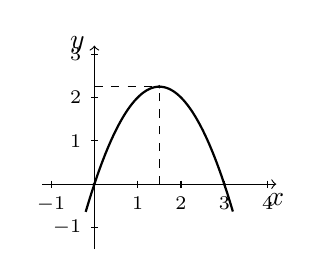
\begin{tikzpicture}[scale=0.55]
    \draw[->] (-1.2,0) -- (4.2,0) node[below] {$x$};
    \draw[->] (0,-1.5) -- (0,3.2) node[left] {$y$};
    \foreach \x in {-1,1,2,3,4}
        \draw (\x,0.08) -- (\x,-0.08) node[below] {\scriptsize $\x$};
    \foreach \y in {-1,1,2,3}
        \draw (0.08,\y) -- (-0.08,\y) node[left] {\scriptsize $\y$};
    \draw[smooth, samples=200, domain=-0.2:3.2, thick] plot (\x, {-(\x)*(\x-3)});
    \fill (0,0) circle (1.2pt);
    \fill (3,0) circle (1.2pt);
    \fill (1.5,2.25) circle (1.2pt);
    \draw[dashed] (1.5,0) -- (1.5,2.25);
    \draw[dashed] (0,2.25) -- (1.5,2.25);
\end{tikzpicture}

\end{center}
Xét các khẳng định sau:
\begin{SubQuestions}
  \TFItem{false}{Hàm số có hai nghiệm là $x=-1$ và $x=4$.}
  \TFItem{true}{Trục đối xứng của đồ thị là đường thẳng $x=\dfrac32$.}
  \TFItem{true}{Hàm số đạt giá trị lớn nhất bằng $2{,}25$.}
  \TFItem{false}{Bất phương trình $f\left(x\right)>0$ có tập nghiệm là $\left[0;3\right]$.}
\end{SubQuestions}
\SolutionBlock{Từ đồ thị, parabol mở xuống và cắt trục hoành tại $x=0$ và $x=3$, nên ý a) sai. Trục đối xứng là đường thẳng đi qua trung điểm hai nghiệm, tức là $x=\dfrac32$, nên ý b) đúng. Đỉnh có tung độ $2{,}25$, nên ý c) đúng. Vì $f\left(x\right)>0$ chỉ khi $0<x<3$, nên ý d) sai.}

\NQuestion Trong mặt phẳng tọa độ $Oxy$, cho $A(2;1),\ B(6;3),\ C(0;5)$. Xét các khẳng định sau:
\begin{SubQuestions}
  \TFItem{true}{$\overrightarrow{AB}=(4;2)$.}
  \TFItem{false}{Trung điểm của đoạn thẳng $BC$ là $I(3;1)$.}
  \TFItem{true}{Đường thẳng $AC$ có phương trình $2x+y-5=0$.}
  \TFItem{false}{Khoảng cách từ điểm $B$ đến đường thẳng $AC$ bằng $\sqrt5$.}
\end{SubQuestions}
\SolutionBlock{\begin{itemize}[leftmargin=1.5em]
\item $\overrightarrow{AB}=(6-2;3-1)=(4;2)$ nên ý a) đúng.
\item Trung điểm của $BC$ là \(\left(\dfrac{6+0}{2};\dfrac{3+5}{2}\right)=(3;4)\), nên ý b) sai.
\item Đường thẳng qua $A(2;1)$ và $C(0;5)$ có hệ số góc \(\dfrac{5-1}{0-2}=-2\), nên phương trình là \(y-1=-2(x-2)\Leftrightarrow 2x+y-5=0\). Ý c) đúng.
\item Khoảng cách từ $B(6;3)$ đến \(AC:2x+y-5=0\) là
\[
\dfrac{|2\cdot6+3-5|}{\sqrt{2^2+1^2}}=\dfrac{10}{\sqrt5}=2\sqrt5\ne \sqrt5.
\]
Nên ý d) sai.
\end{itemize}}
